\documentclass[twoside, pagesize, fontsize=11pt, dvipsnames]{scrreport} %
\usepackage[ngerman]{babel}
\usepackage{anyfontsize} % jede Schriftgrösse eben
\usepackage[table]{xcolor}
\usepackage{tabu}
\usepackage{svg}
\usepackage{fontenc}
\usepackage{eurosym}
\usepackage{soul}           %% Sperren und Schafe stehlen

 \usepackage{enumerate}      %% Nummerieren
 \usepackage{ifthen}         %% Wenn-Dann eben
 \usepackage{array}          %% besserer Mathesatz
 \usepackage[fleqn,reqno]{amsmath}            %% für Mathematiksatz
 \usepackage{amssymb}           %% für Symbole

 \usepackage{marginnote}        %% Randnotizen (für Hypref)
 \usepackage{booktabs}          %% bessere Linien in Tabellen
 \usepackage{longtable}
 \usepackage{makecell}
\usepackage{graphicx}
 \usepackage{float}             %% Gleitobjektumgebungen
 \usepackage{flafter}           %% floats hinter ersten Verweis
 \usepackage{rotfloat, rotating}      %% drehen
 \usepackage{morefloats}    %% erweitert die Möglichkeiten

\usepackage[most]{tcolorbox}

 \usepackage{titletoc}
 \usepackage{afterpage}

 \usepackage{hanging}
 \usepackage{natbib}
%\bibliographystyle{apalike}
% \usepackage{babelbib}
% \usepackage{bibgerm}

%% für huxtables
\usepackage{calc}
%\usepackage{tabularx}
\usepackage{threeparttable}
% ende für huxtables
\usepackage{wrapfig}
 \usepackage{fancybox}          %% Schöne Boxen
 \usepackage{nameref}
 \usepackage[ngerman]{varioref}

 \usepackage{pdfpages}
 \usepackage{setspace}
 \usepackage{boxedminipage}     %% umrahmte Boxen
 \usepackage{multicol}          %% mehrspaltige Zeilen
 \usepackage{epsfig,lscape}     %% Graphiken auch Quer

\usepackage[stable, norule, flushmargin]{footmisc} %% Fußgut

 \usepackage[np]{numprint}  %%Zahlen an Komma ausrichten

 \usepackage[mla]{ellipsis}       %% Auslassungspunkte
% \usepackage[newcommands]{ragged2e} %Verbesserung der Seitenaufteilung
 \usepackage[safe]{textcomp} %zusätzliche Zeichen, wie schwarze Punkte

%%%% hyperref %%%%
\usepackage[hyphens]{url} %% URLs sauber einfügen und umbrechen - muss vor hyperref
\usepackage[pdfa=true, pdflang = de, colorlinks = true, allcolors = darkgray]{hyperref}
%%%% muss alles hinter hyperref, weil es sonst package-clashes erzeugt:
\usepackage{accsupp}    %% für Barrierefreiheit
\usepackage{pdfcomment} %% für Barrierefreiheit
%\PassOptionsToPackage{hyphens}{accsupp} %% übergibt hyphens für das url-Paket, das in accsupp ohne diese Option geladen wird.
\PassOptionsToPackage{hyphens}{pdfcomment} %% übergibt hyphens für das url-Paket, das in pdfcomment ohne diese Option geladen wird.
%%%%

\usepackage{twoopt}

\usepackage{paralist}
\usepackage{siunitx}

\usepackage{pdflscape}

\usepackage{colortbl}

%\usepackage[style=authoryear,maxcitenames=2, backend=biber, isbn=false,doi=false, eprint = false]{biblatex}

%___________________  Pakete Ende  ____________________________________________


\usepackage{color}
\usepackage{fancyvrb}
\newcommand{\VerbBar}{|}
\newcommand{\VERB}{\Verb[commandchars=\\\{\}]}
\DefineVerbatimEnvironment{Highlighting}{Verbatim}{commandchars=\\\{\}}
% Add ',fontsize=\small' for more characters per line
\usepackage{framed}
\definecolor{shadecolor}{RGB}{241,243,245}
\newenvironment{Shaded}{\begin{snugshade}}{\end{snugshade}}
\newcommand{\AlertTok}[1]{\textcolor[rgb]{0.68,0.00,0.00}{#1}}
\newcommand{\AnnotationTok}[1]{\textcolor[rgb]{0.37,0.37,0.37}{#1}}
\newcommand{\AttributeTok}[1]{\textcolor[rgb]{0.40,0.45,0.13}{#1}}
\newcommand{\BaseNTok}[1]{\textcolor[rgb]{0.68,0.00,0.00}{#1}}
\newcommand{\BuiltInTok}[1]{\textcolor[rgb]{0.00,0.23,0.31}{#1}}
\newcommand{\CharTok}[1]{\textcolor[rgb]{0.13,0.47,0.30}{#1}}
\newcommand{\CommentTok}[1]{\textcolor[rgb]{0.37,0.37,0.37}{#1}}
\newcommand{\CommentVarTok}[1]{\textcolor[rgb]{0.37,0.37,0.37}{\textit{#1}}}
\newcommand{\ConstantTok}[1]{\textcolor[rgb]{0.56,0.35,0.01}{#1}}
\newcommand{\ControlFlowTok}[1]{\textcolor[rgb]{0.00,0.23,0.31}{#1}}
\newcommand{\DataTypeTok}[1]{\textcolor[rgb]{0.68,0.00,0.00}{#1}}
\newcommand{\DecValTok}[1]{\textcolor[rgb]{0.68,0.00,0.00}{#1}}
\newcommand{\DocumentationTok}[1]{\textcolor[rgb]{0.37,0.37,0.37}{\textit{#1}}}
\newcommand{\ErrorTok}[1]{\textcolor[rgb]{0.68,0.00,0.00}{#1}}
\newcommand{\ExtensionTok}[1]{\textcolor[rgb]{0.00,0.23,0.31}{#1}}
\newcommand{\FloatTok}[1]{\textcolor[rgb]{0.68,0.00,0.00}{#1}}
\newcommand{\FunctionTok}[1]{\textcolor[rgb]{0.28,0.35,0.67}{#1}}
\newcommand{\ImportTok}[1]{\textcolor[rgb]{0.00,0.46,0.62}{#1}}
\newcommand{\InformationTok}[1]{\textcolor[rgb]{0.37,0.37,0.37}{#1}}
\newcommand{\KeywordTok}[1]{\textcolor[rgb]{0.00,0.23,0.31}{#1}}
\newcommand{\NormalTok}[1]{\textcolor[rgb]{0.00,0.23,0.31}{#1}}
\newcommand{\OperatorTok}[1]{\textcolor[rgb]{0.37,0.37,0.37}{#1}}
\newcommand{\OtherTok}[1]{\textcolor[rgb]{0.00,0.23,0.31}{#1}}
\newcommand{\PreprocessorTok}[1]{\textcolor[rgb]{0.68,0.00,0.00}{#1}}
\newcommand{\RegionMarkerTok}[1]{\textcolor[rgb]{0.00,0.23,0.31}{#1}}
\newcommand{\SpecialCharTok}[1]{\textcolor[rgb]{0.37,0.37,0.37}{#1}}
\newcommand{\SpecialStringTok}[1]{\textcolor[rgb]{0.13,0.47,0.30}{#1}}
\newcommand{\StringTok}[1]{\textcolor[rgb]{0.13,0.47,0.30}{#1}}
\newcommand{\VariableTok}[1]{\textcolor[rgb]{0.07,0.07,0.07}{#1}}
\newcommand{\VerbatimStringTok}[1]{\textcolor[rgb]{0.13,0.47,0.30}{#1}}
\newcommand{\WarningTok}[1]{\textcolor[rgb]{0.37,0.37,0.37}{\textit{#1}}}

%\def\tightlist{}

%%%%%%%%%%%%%%%%%%%%%  Größen ändern gegen LaTeXs Hysterie %%%%%%%%%%%%%%%%%%%%%%%%%%%%%%
\widowpenalty=10000 % erschwert Hurenkindern das Leben
\clubpenalty=3000 % erschwert Schusterjungen das Leben
\tolerance=300  %Wortabstände dehnbarer; fürs Final auf 300!!
\hbadness= 300
  \emergencystretch= 1.5em
 \hfuzz = 0.3pt
 \vfuzz \hfuzz
 \raggedbottom

%% erste Zeile einrücken
\setlength{\parindent}{1em}
\newcommand{\Absatz}{\vspace{4ex} \noindent}

%% Einzug für Formeln
\setlength\mathindent{1pc}
%% Fußnoten
%\counterwithout{footnote}{chapter} % über Kapitel hinweg zählen
\addtolength{\skip\footins}{1ex plus 2mm} % Abstand zum Text
\renewcommand{\footnotesep}{1ex} % da nummeriert, Abstand ok
% rechtsbündig aus likem Rand

\let\Umathcode\XeTeXmathcode \let\Umathchardef\XeTeXmathchardef

%____________ Größen Ende ______________________________

%%%%% Farbboxen für Hinweise ------
\tcbset{textmarker/.style={%
        enhanced,
        parbox=false,boxrule=0mm,boxsep=0mm,arc=0mm,
        outer arc=0mm,left=6mm,right=3mm,top=7pt,bottom=7pt,
        toptitle=1mm,bottomtitle=1mm,oversize}}

\newtcolorbox{hintBox}{textmarker,
    borderline west={6pt}{0pt}{yellow},
    colback=yellow!10!white}

\newtcolorbox{importantBox}{textmarker,
    borderline west={6pt}{0pt}{red},
    colback=red!10!white}

\newtcolorbox{noteBox}{textmarker,
    borderline west={6pt}{0pt}{green},
    colback=green!10!white}

\newcommand{\Anmerkung}[1]
{\begin{hintBox}
#1
\end{hintBox}}

\newcommand{\Alarm}[1]
{\begin{importantBox}
#1
\end{importantBox}}

\newcommand{\Allesgut}[1]
{\begin{noteBox}
#1
\end{noteBox}}


\newcommand{\on}[1]{{#1}} %deaktiviertes oldstylenums
\newcommand{\p}{{\npnoaddmissingzero \npdecimalsign{.}}} %p-Wert
                                %kompakt in zB Kovarianztabellen

%%%%%%%%%      Umgebungen und Kommandos   %%%%%%%%%%%%%%%%%%%%%%%%%%%%

%%%%  Boxen

\newtcolorbox{IYI_C}{
  colback=white,
  colframe=MidnightBlue,
  coltext=black,
  boxsep=5pt,
  arc=4pt}

\newenvironment{IYI}[1]
  {
  \begin{itemize}
  \renewcommand{\labelitemi}{
    \raisebox{-.9\height}[0pt][0pt]{
      {\setkeys{Gin}{width= 3em,keepaspectratio}
        \hspace*{-3cm}
\includegraphics{images/IYI.pdf}}
    }
  }
  \setlength{\fboxsep}{1em}
  \begin{IYI_C}
  \item
  }
  {
  \end{IYI_C}
  \end{itemize}
  }

\newtcolorbox{QA_C}{
  colback=white,
  colframe=orange,
  coltext=black,
  boxsep=5pt,
  arc=4pt}

  \newenvironment{QA}[1]
  {
  \begin{itemize}
  \renewcommand{\labelitemi}{
    \raisebox{-.9\height}[0pt][0pt]{
      {\setkeys{Gin}{width=3em,keepaspectratio}
        \hspace{-2cm}
\includegraphics{images/QA.pdf}}
    }
  }
  \setlength{\fboxsep}{1em}
  \begin{QA_C}
  \item
  }
  {
  \end{QA_C}
  \end{itemize}
  }

%%% ENDE Boxen

%% \PBS für geschützten Backslash
\newcommand{\PreserveBackslash}[1]{\let\temp=\\#1\let\\=\temp}
\let\PBS=\PreserveBackslash

\renewcommand{\labelitemi}{--}

%%% Bilder einbauen (breitbild = Seitenbreite skalieren; bild zentriert
\newcommandtwoopt{\Bild}[3][1][0 0 0
0]{ \begin{center}
    \includegraphics[width=#1\linewidth,trim = #2, clip]{images/#3}
  \end{center}}
%%%% Aufzählungen

\renewcommand{\labelitemi}{\small\textbullet}

\newcommand{\Beschrieb}[1]{\ifthenelse{\isundefined{#1}}{}{
\begin{minipage}[H]{1.0\linewidth}
  \begin{multicols}{3}
 #1
 \end{multicols}
\end{minipage}\vspace{5mm}}}

%% für Barrierefreiheit
\newcommand{\AccTool}[2]{\BeginAccSupp{method=pdfstringdef,unicode,Alt={{#1}}}\pdftooltip{{#2}}{{#1}}\EndAccSupp{}}

%__________________ Umgebungen Ende _____________________________________________

%--------  Tabellenbefehle  ----------------------
%LaTeX interpretiert Tabulatoren und Zeilenenden für Tabellen
% & und \\ können eingesetzt werden, wenn nötig
% bei zB \\\midrule%! muss das Zeilenende auskommentiert sein

\renewcommand{\floatpagefraction}{.7}
\renewcommand{\textfraction}{.12}
\renewcommand{\topfraction}{.8}     % vorher: .7
\renewcommand{\bottomfraction}{.5}  % vorher: .3
\makeatletter
\renewcommand{\fps@figure}{htbp}
\renewcommand{\fps@table}{htbp}
\makeatother

\setbox0=\hbox{%
  \begin{tabular}{c}
 \global\let\CsvNewline\\%
 \end{tabular}}
 {\catcode`\^^M=\active%
  \gdef\CsvObeylines{\catcode`\^^M=\active \let^^M=\CsvNewline}}%

\setcapindent{1em}

\newcommand{\TBZeilenabstand}{\aboverulesep = 0pt \belowrulesep = 0pt}

\newcommand{\NormalZeilenabstand}{\aboverulesep = 0.605mm \belowrulesep = 0.984mm}


% \newcommand{\corcmidrule}[1][2pt]{% \corcmidrule[<len>]
%   \\[\dimexpr-\normalbaselineskip-\belowrulesep-\aboverulesep-#1\relax]%
% }

% Correct for \cmidrule colour adjustment/vertical skip
\newcommand{\corcmidrule}[1][2pt]{% \corcmidrule[<len>]
  \\[\dimexpr-\arraystretch\normalbaselineskip-\belowrulesep-\aboverulesep-#1\relax]%
}

 \newcommand{\cgrauDurch}{\arrayrulecolor{black!30}\specialrule{.2pt}{0pt}{0pt}\arrayrulecolor{black}}
 \newcommand{\cgrau}[1]{\arrayrulecolor{black!30} \cmidrule[.8pt](l{3pt}r{2pt}){#1} \corcmidrule[1pt] \arrayrulecolor{black}}

%% variable Verweise
\renewcommand\reftextfaceafter{gegen\"uberliegend}
\renewcommand\reftextfacebefore{gegen\"uberliegend}
\renewcommand\reftextbefore{vorherige Seite}
\renewcommand\reftextafter{n\"achste Seite}
\renewcommand\reftextcurrent{}
\renewcommand\reftextfaraway[1]{Seite~\pageref{#1}}

\makeatletter
\@addtoreset{figure}{section}
\@addtoreset{table}{section}
\makeatother

\renewcommand{\thefigure}{\thesection.\arabic{figure}}
\renewcommand{\thetable}{\thesection.\arabic{table}}

%\renewcommand{\bminipage}{\begin{minipage}[t]{.9\textwidth}}
%\renewcommand{\eminipage}{\end{minipage}}

%%%%%%%%%%%%%%%%%%%%%%%%%%%%%%%%%%%%%%%%%%%%%%%%
%    aus Bookdown
%%%%%%%%%%%%%%%%%%%%%%%%%%%%%%%%%%%%%%%%%%%%%%%%
%
\definecolor{shadecolor}{RGB}{248,248,248}
% \newenvironment{Shaded}{\begin{snugshade}}{\end{snugshade}}
%\newcommand{\AlertTok}[1]{\textcolor[rgb]{0.94,0.16,0.16}{#1}}
% \newcommand{\AnnotationTok}[1]{\textcolor[rgb]{0.56,0.35,0.01}{\textbf{\textit{#1}}}}
% \newcommand{\AttributeTok}[1]{\textcolor[rgb]{0.77,0.63,0.00}{#1}}
% \newcommand{\BaseNTok}[1]{\textcolor[rgb]{0.00,0.00,0.81}{#1}}
% \newcommand{\BuiltInTok}[1]{#1}
% \newcommand{\CharTok}[1]{\textcolor[rgb]{0.31,0.60,0.02}{#1}}
% \newcommand{\CommentTok}[1]{\textcolor[rgb]{0.56,0.35,0.01}{\textit{#1}}}
% \newcommand{\CommentVarTok}[1]{\textcolor[rgb]{0.56,0.35,0.01}{\textbf{\textit{#1}}}}
% \newcommand{\ConstantTok}[1]{\textcolor[rgb]{0.00,0.00,0.00}{#1}}
% \newcommand{\ControlFlowTok}[1]{\textcolor[rgb]{0.13,0.29,0.53}{\textbf{#1}}}
% \newcommand{\DataTypeTok}[1]{\textcolor[rgb]{0.13,0.29,0.53}{#1}}
% \newcommand{\DecValTok}[1]{\textcolor[rgb]{0.00,0.00,0.81}{#1}}
% \newcommand{\DocumentationTok}[1]{\textcolor[rgb]{0.56,0.35,0.01}{\textbf{\textit{#1}}}}
% \newcommand{\ErrorTok}[1]{\textcolor[rgb]{0.64,0.00,0.00}{\textbf{#1}}}
% \newcommand{\ExtensionTok}[1]{#1}
% \newcommand{\FloatTok}[1]{\textcolor[rgb]{0.00,0.00,0.81}{#1}}
% \newcommand{\FunctionTok}[1]{\textcolor[rgb]{0.00,0.00,0.00}{#1}}
% \newcommand{\ImportTok}[1]{#1}
% \newcommand{\InformationTok}[1]{\textcolor[rgb]{0.56,0.35,0.01}{\textbf{\textit{#1}}}}
% \newcommand{\KeywordTok}[1]{\textcolor[rgb]{0.13,0.29,0.53}{\textbf{#1}}}
% \newcommand{\NormalTok}[1]{#1}
% \newcommand{\OperatorTok}[1]{\textcolor[rgb]{0.81,0.36,0.00}{\textbf{#1}}}
% \newcommand{\OtherTok}[1]{\textcolor[rgb]{0.56,0.35,0.01}{#1}}
% \newcommand{\PreprocessorTok}[1]{\textcolor[rgb]{0.56,0.35,0.01}{\textit{#1}}}
% \newcommand{\RegionMarkerTok}[1]{#1}
% \newcommand{\SpecialCharTok}[1]{\textcolor[rgb]{0.00,0.00,0.00}{#1}}
% \newcommand{\SpecialStringTok}[1]{\textcolor[rgb]{0.31,0.60,0.02}{#1}}
% \newcommand{\StringTok}[1]{\textcolor[rgb]{0.31,0.60,0.02}{#1}}
% \newcommand{\VariableTok}[1]{\textcolor[rgb]{0.00,0.00,0.00}{#1}}
% \newcommand{\VerbatimStringTok}[1]{\textcolor[rgb]{0.31,0.60,0.02}{#1}}
% \newcommand{\WarningTok}[1]{\textcolor[rgb]{0.56,0.35,0.01}{\textbf{\textit{#1}}}}

\makeatletter
\def\maxwidth{\ifdim\Gin@nat@width>\linewidth\linewidth\else\Gin@nat@width\fi}
\def\maxheight{\ifdim\Gin@nat@height>\textheight\textheight\else\Gin@nat@height\fi}
\makeatother

\providecommand{\tightlist}{%
  \setlength{\itemsep}{0pt}\setlength{\parskip}{0pt}}
\setcounter{secnumdepth}{5}

\ifx\paragraph\undefined\else
\let\oldparagraph\paragraph
\renewcommand{\paragraph}[1]{\oldparagraph{#1}\mbox{}}
\fi
\ifx\subparagraph\undefined\else
\let\oldsubparagraph\subparagraph
\renewcommand{\subparagraph}[1]{\oldsubparagraph{#1}\mbox{}}
\fi

%%% Use protect on footnotes to avoid problems with footnotes in titles
\let\rmarkdownfootnote\footnote%
\def\footnote{\protect\rmarkdownfootnote}

%%% Change title format to be more compact
\usepackage{titling}

%%%%%%%%%%%%%%%%%%%%%%%%%%%% aus bookdown Ende %%%%%%%%%%%%%%%%%%%%%%%%%%%%%%%%%%%%%%%%%%%


\hypersetup {pdflang = de, colorlinks = true, linkcolor =
  black, urlcolor = black, pdfauthor={Dr. Fretwurst, Benjamin},
  pdfsubject={Statistik Aufbau}, pdftitle={Wissen macht R!},
  pdfkeywords={Statistik, lineares Modell, Regression, Varianzanalyse, Clusteranalyse} lang = {DE} }
\urlstyle{same}

%\addbibresource{../PeM.bib}
%\ExecuteBibliographyOptions{url=true, doi = false}

\usepackage[a4paper, left=30mm, asymmetric, top=30mm,textwidth=15cm,
textheight=22.5cm]{geometry}

% Headers and footers
\usepackage{scrlayer-scrpage}
\pagestyle{scrheadings}

  \clearscrheadfoot
 \automark[section]{section}
  \ihead[]{\headmark} %oben links
  \chead[]{} %oben Mitte
  \ohead{\pagemark} %oben rechts Logo über AddToShipoutPicture unten
  \ifoot[]{\footnotesize{}} %unten links
  \cfoot[]{} %unten Mitte
  \ofoot[]{\footnotesize{}} % unten rechts
  \setheadsepline{.2pt}
  \setfootsepline{.2pt}
\addtokomafont{disposition}{\sffamily}

\addtokomafont{disposition}{\sffamily}
%\renewcommand{\familydefault}{\sfdefault}

\usepackage[labelsep=colon]{caption}
% \captionsetup[table]{textfont = {sf}, labelfont = {sf}} %bf
%\renewcaptionname{ngerman}{\tablename}{Tabelle}

%\usepackage{baskervald} % auch nicht schlecht
\usepackage[]{CrimsonPro} % gut
%\setmainfont{Century Gothic} %schlimm, aber IaKom und darum schön

%\usepackage[german=swiss]{csquotes}

%%%%%%%%%%%%%%%%%%%%%%%%%%%%%%%%%%%%%%%%%%%%

              %Dokumentstart

%%%%%%%%%%%%%%%%%%%%%%%%%%%%%%%%%%%%%%%%%%%%

\hyphenation{
al-ler-dings
Al-ters-grup-pen
Be-reich
Co-ro-na-kri-se
Fern-seh-an-ge-bo-te
Fern-seh-ge-rät
Fern-seh-ge-rä-te
Fest-netz-tele-fo-nie
Ge-samt-zu-frie-den-heit
glei-chen
glei-chen
In-for-ma-tions-suche
in-nen
ita-li-e-nische
je-weils
po-li-ti-schem
po-li-ti-schen
si-tu-a-ti-ve
si-tu-a-tiv
Sta-bi-li-tät
Ver-schwö-rungs-theo-re-ti-ker
Ver-trau-ens-kluft
Zeit-um-fänge
Zu-schau-er
zweit-höchs-ten
}

\begin{document}

\begin{titlepage}
\sffamily
\setlength\parindent{0pt}

\hfill 
\includegraphics[width = 6cm]{../images/uzh_logo_d_pos.pdf}\par

\vspace{5cm}


{\bfseries \fontsize{20}{26} \selectfont Wissen macht R!} \\[1ex]


\vfill

Dr. Benjamin Fretwurst\\

\vfill
{\large }
\raggedright



1/9/23 \\[.5cm]
%\textbf{[\today] \\[1.5cm]}
\pagenumbering{Roman}
\clearpage

\vspace*{4cm}

Quellenangabe\\[.5cm]



%\end{tabbing}
\end{titlepage}


\makeatletter
\AddToShipoutPicture{\setlength{\unitlength}{1cm}\put(24.32,18.65){{
\includegraphics[height=.6cm]{../images/uzh_logo_d_pos.pdf}}}}
\makeatletter

%Überschriften unterdrücken durch IV und TV (wegen multicolumn)
\renewcommand{\listoftables}{\@starttoc{lot}}
\renewcommand{\tableofcontents}{\@starttoc{toc}}
\renewcommand{\listoffigures}{\@starttoc{lof}}

%Mehr Platz für breite Tabellennummern
\renewcommand{\l@table}{\@dottedtocline{1}{1em}{3em}}
\makeatother

\clearpage
\section*{Inhalt}
\label{sec:inhalt}
\pdfbookmark[1]{\contentsname}{toc}
%  \begin{multicols}{2}

\tableofcontents
%  \end{multicols}

\clearpage

\section*{Tabellen- und Abbildungsverzeichnis}

\pdfbookmark[1]{Tabellen/Abbildungen}{lot}

\section*{Abbildungsverzeichnis}
\label{sec:Abbildungsverzeichnis}

%\begin{multicols}{2}
\listoffigures
%\end{multicols}

\section*{Tabellenverzeichnis}
\label{sec:tabellenverzeichnis}

%\begin{multicols}{2}
\listoftables
%\end{multicols}

\cleardoublepage

\pagenumbering{arabic}
%%%%%%%%%%%%%%%%%%%%%%%%%%%%%%%%%%

             %Body

%%%%%%%%%%%%%%%%%%%%%%%%%%%%%%%%%%

\bookmarksetup{startatroot}

\hypertarget{intro}{%
\chapter*{Intro}\label{intro}}
\addcontentsline{toc}{chapter}{Intro}

\markboth{Intro}{Intro}

Dieser Style Guide umfasst Empfehlungen, die die Arbeit mit R etwas
vereinheitlichen soll, wo es sinnvoll erscheint, damit in der Lehre und
in Projekten gut zusammengearbeitet werden kann und nicht alles immer zu
fremd aussieht.

Two R packages support this style guide:

\begin{itemize}
\item
  \href{http://styler.r-lib.org}{styler} allows you to interactively
  restyle selected text, files, or entire projects. It includes an
  RStudio add-in, the easiest way to re-style existing code.

  \begin{figure}

  {\centering 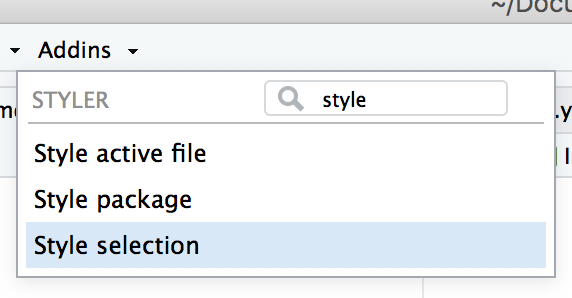
\includegraphics[width=2.6in,height=\textheight]{styler-addin.png}

  }

  \end{figure}
\item
  \href{https://github.com/jimhester/lintr}{lintr} performs automated
  checks to confirm that you conform to the style guide.
\end{itemize}

\bookmarksetup{startatroot}

\hypertarget{files}{%
\chapter{Files}\label{files}}

\hypertarget{names}{%
\section{Names}\label{names}}

File names should be meaningful and end in \texttt{.R}. Avoid using
special characters in file names - stick with numbers, letters,
\texttt{-}, and \texttt{\_}.

\begin{verbatim}
# Good
fit_models.R
utility_functions.R

# Bad
fit models.R
foo.r
stuff.r
\end{verbatim}

If files should be run in a particular order, prefix them with numbers.
If it seems likely you'll have more than 10 files, left pad with zero:

\begin{verbatim}
00_download.R
01_explore.R
...
09_model.R
10_visualize.R
\end{verbatim}

If you later realise that you've missed some steps, it's tempting to use
\texttt{02a}, \texttt{02b}, etc. However, I think it's generally better
to bite the bullet and rename all files.

Pay attention to capitalization, since you, or some of your
collaborators, might be using an operating system with a
case-insensitive file system (e.g., Microsoft Windows or OS X) which can
lead to problems with (case-sensitive) revision control systems. Prefer
file names that are all lower case, and never have names that differ
only in their capitalization.

\hypertarget{organisation}{%
\section{Organisation}\label{organisation}}

It's hard to describe exactly how you should organise your code across
multiple files. I think the best rule of thumb is that if you can give a
file a concise name that still evokes its contents, you've arrived at a
good organisation. But getting to that point is hard.

\hypertarget{internal-structure}{%
\section{Internal structure}\label{internal-structure}}

Use commented lines of \texttt{-} and \texttt{=} to break up your file
into easily readable chunks.

\begin{Shaded}
\begin{Highlighting}[]
\CommentTok{\# Load data {-}{-}{-}{-}{-}{-}{-}{-}{-}{-}{-}{-}{-}{-}{-}{-}{-}{-}{-}{-}{-}{-}{-}{-}{-}{-}{-}}

\CommentTok{\# Plot data {-}{-}{-}{-}{-}{-}{-}{-}{-}{-}{-}{-}{-}{-}{-}{-}{-}{-}{-}{-}{-}{-}{-}{-}{-}{-}{-}}
\end{Highlighting}
\end{Shaded}

If your script uses add-on packages, load them all at once at the very
beginning of the file. This is more transparent than sprinkling
\texttt{library()} calls throughout your code or having hidden
dependencies that are loaded in a startup file, such as
\texttt{.Rprofile}.

\bookmarksetup{startatroot}

\hypertarget{syntax}{%
\chapter{Syntax}\label{syntax}}

\hypertarget{object-names}{%
\section{Object names}\label{object-names}}

\begin{quote}
\enquote{There are only two hard things in Computer Science: cache
invalidation and naming things.}

--- Phil Karlton
\end{quote}

Variable and function names should use only lowercase letters, numbers,
and \texttt{\_}. Use underscores (\texttt{\_}) (so called snake case) to
separate words within a name.

\begin{Shaded}
\begin{Highlighting}[]
\CommentTok{\# Good}
\NormalTok{day\_one}
\NormalTok{day\_1}

\CommentTok{\# Bad}
\NormalTok{DayOne}
\NormalTok{dayone}
\end{Highlighting}
\end{Shaded}

Base R uses dots in function names (\texttt{contrib.url()}) and class
names (\texttt{data.frame}), but it's better to reserve dots exclusively
for the S3 object system. In S3, methods are given the name
\texttt{function.class}; if you also use \texttt{.} in function and
class names, you end up with confusing methods like
\texttt{as.data.frame.data.frame()}.

If you find yourself attempting to cram data into variable names
(e.g.~\texttt{model\_2018}, \texttt{model\_2019}, \texttt{model\_2020}),
consider using a list or data frame instead.

Generally, variable names should be nouns and function names should be
verbs. Strive for names that are concise and meaningful (this is not
easy!).

\begin{Shaded}
\begin{Highlighting}[]
\CommentTok{\# Good}
\NormalTok{day\_one}

\CommentTok{\# Bad}
\NormalTok{first\_day\_of\_the\_month}
\NormalTok{djm1}
\end{Highlighting}
\end{Shaded}

Where possible, avoid re-using names of common functions and variables.
This will cause confusion for the readers of your code.

\begin{Shaded}
\begin{Highlighting}[]
\CommentTok{\# Bad}
\NormalTok{T }\OtherTok{\textless{}{-}} \ConstantTok{FALSE}
\NormalTok{c }\OtherTok{\textless{}{-}} \DecValTok{10}
\NormalTok{mean }\OtherTok{\textless{}{-}} \ControlFlowTok{function}\NormalTok{(x) }\FunctionTok{sum}\NormalTok{(x)}
\end{Highlighting}
\end{Shaded}

\hypertarget{spacing}{%
\section{Spacing}\label{spacing}}

\hypertarget{commas}{%
\subsection{Commas}\label{commas}}

Always put a space after a comma, never before, just like in regular
English.

\begin{Shaded}
\begin{Highlighting}[]
\CommentTok{\# Good}
\NormalTok{x[, }\DecValTok{1}\NormalTok{]}

\CommentTok{\# Bad}
\NormalTok{x[,}\DecValTok{1}\NormalTok{]}
\NormalTok{x[ ,}\DecValTok{1}\NormalTok{]}
\NormalTok{x[ , }\DecValTok{1}\NormalTok{]}
\end{Highlighting}
\end{Shaded}

\hypertarget{parentheses}{%
\subsection{Parentheses}\label{parentheses}}

Do not put spaces inside or outside parentheses for regular function
calls.

\begin{Shaded}
\begin{Highlighting}[]
\CommentTok{\# Good}
\FunctionTok{mean}\NormalTok{(x, }\AttributeTok{na.rm =} \ConstantTok{TRUE}\NormalTok{)}

\CommentTok{\# Bad}
\FunctionTok{mean}\NormalTok{ (x, }\AttributeTok{na.rm =} \ConstantTok{TRUE}\NormalTok{)}
\FunctionTok{mean}\NormalTok{( x, }\AttributeTok{na.rm =} \ConstantTok{TRUE}\NormalTok{ )}
\end{Highlighting}
\end{Shaded}

Place a space before and after \texttt{()} when used with \texttt{if},
\texttt{for}, or \texttt{while}.

\begin{Shaded}
\begin{Highlighting}[]
\CommentTok{\# Good}
\ControlFlowTok{if}\NormalTok{ (debug) \{}
  \FunctionTok{show}\NormalTok{(x)}
\NormalTok{\}}

\CommentTok{\# Bad}
\ControlFlowTok{if}\NormalTok{(debug)\{}
  \FunctionTok{show}\NormalTok{(x)}
\NormalTok{\}}
\end{Highlighting}
\end{Shaded}

Place a space after \texttt{()} used for function arguments:

\begin{Shaded}
\begin{Highlighting}[]
\CommentTok{\# Good}
\ControlFlowTok{function}\NormalTok{(x) \{\}}

\CommentTok{\# Bad}
\ControlFlowTok{function}\NormalTok{ (x) \{\}}
\ControlFlowTok{function}\NormalTok{(x)\{\}}
\end{Highlighting}
\end{Shaded}

\hypertarget{embracing}{%
\subsection{Embracing}\label{embracing}}

The embracing operator, \texttt{\{\{\ \}\}}, should always have inner
spaces to help emphasise its special behaviour:

\begin{Shaded}
\begin{Highlighting}[]
\CommentTok{\# Good}
\NormalTok{max\_by }\OtherTok{\textless{}{-}} \ControlFlowTok{function}\NormalTok{(data, var, by) \{}
\NormalTok{  data }\SpecialCharTok{\%\textgreater{}\%}
    \FunctionTok{group\_by}\NormalTok{(\{\{ by \}\}) }\SpecialCharTok{\%\textgreater{}\%}
    \FunctionTok{summarise}\NormalTok{(}\AttributeTok{maximum =} \FunctionTok{max}\NormalTok{(\{\{ var \}\}, }\AttributeTok{na.rm =} \ConstantTok{TRUE}\NormalTok{))}
\NormalTok{\}}

\CommentTok{\# Bad}
\NormalTok{max\_by }\OtherTok{\textless{}{-}} \ControlFlowTok{function}\NormalTok{(data, var, by) \{}
\NormalTok{  data }\SpecialCharTok{\%\textgreater{}\%}
    \FunctionTok{group\_by}\NormalTok{(\{\{by\}\}) }\SpecialCharTok{\%\textgreater{}\%}
    \FunctionTok{summarise}\NormalTok{(}\AttributeTok{maximum =} \FunctionTok{max}\NormalTok{(\{\{var\}\}, }\AttributeTok{na.rm =} \ConstantTok{TRUE}\NormalTok{))}
\NormalTok{\}}
\end{Highlighting}
\end{Shaded}

\hypertarget{infix-operators}{%
\subsection{Infix operators}\label{infix-operators}}

Most infix operators (\texttt{==}, \texttt{+}, \texttt{-},
\texttt{\textless{}-}, etc.) should always be surrounded by spaces:

\begin{Shaded}
\begin{Highlighting}[]
\CommentTok{\# Good}
\NormalTok{height }\OtherTok{\textless{}{-}}\NormalTok{ (feet }\SpecialCharTok{*} \DecValTok{12}\NormalTok{) }\SpecialCharTok{+}\NormalTok{ inches}
\FunctionTok{mean}\NormalTok{(x, }\AttributeTok{na.rm =} \ConstantTok{TRUE}\NormalTok{)}

\CommentTok{\# Bad}
\NormalTok{height}\OtherTok{\textless{}{-}}\NormalTok{feet}\SpecialCharTok{*}\DecValTok{12}\SpecialCharTok{+}\NormalTok{inches}
\FunctionTok{mean}\NormalTok{(x, }\AttributeTok{na.rm=}\ConstantTok{TRUE}\NormalTok{)}
\end{Highlighting}
\end{Shaded}

There are a few exceptions, which should never be surrounded by spaces:

\begin{itemize}
\item
  The operators with \href{https://rdrr.io/r/base/Syntax.html}{high
  precedence}: \texttt{::}, \texttt{:::}, \texttt{\$}, \texttt{@},
  \texttt{{[}}, \texttt{{[}{[}}, \texttt{\^{}}, unary \texttt{-}, unary
  \texttt{+}, and \texttt{:}.

\begin{Shaded}
\begin{Highlighting}[]
\CommentTok{\# Good}
\FunctionTok{sqrt}\NormalTok{(x}\SpecialCharTok{\^{}}\DecValTok{2} \SpecialCharTok{+}\NormalTok{ y}\SpecialCharTok{\^{}}\DecValTok{2}\NormalTok{)}
\NormalTok{df}\SpecialCharTok{$}\NormalTok{z}
\NormalTok{x }\OtherTok{\textless{}{-}} \DecValTok{1}\SpecialCharTok{:}\DecValTok{10}

\CommentTok{\# Bad}
\FunctionTok{sqrt}\NormalTok{(x }\SpecialCharTok{\^{}} \DecValTok{2} \SpecialCharTok{+}\NormalTok{ y }\SpecialCharTok{\^{}} \DecValTok{2}\NormalTok{)}
\NormalTok{df }\SpecialCharTok{$}\NormalTok{ z}
\NormalTok{x }\OtherTok{\textless{}{-}} \DecValTok{1} \SpecialCharTok{:} \DecValTok{10}
\end{Highlighting}
\end{Shaded}
\item
  Single-sided formulas when the right-hand side is a single identifier:

\begin{Shaded}
\begin{Highlighting}[]
\CommentTok{\# Good}
\SpecialCharTok{\textasciitilde{}}\NormalTok{foo}
\FunctionTok{tribble}\NormalTok{(}
  \SpecialCharTok{\textasciitilde{}}\NormalTok{col1, }\SpecialCharTok{\textasciitilde{}}\NormalTok{col2,}
  \StringTok{"a"}\NormalTok{,   }\StringTok{"b"}
\NormalTok{)}

\CommentTok{\# Bad}
\SpecialCharTok{\textasciitilde{}}\NormalTok{ foo}
\FunctionTok{tribble}\NormalTok{(}
  \SpecialCharTok{\textasciitilde{}}\NormalTok{ col1, }\SpecialCharTok{\textasciitilde{}}\NormalTok{ col2,}
  \StringTok{"a"}\NormalTok{, }\StringTok{"b"}
\NormalTok{)}
\end{Highlighting}
\end{Shaded}

  Note that single-sided formulas with a complex right-hand side do need
  a space:

\begin{Shaded}
\begin{Highlighting}[]
\CommentTok{\# Good}
\SpecialCharTok{\textasciitilde{}}\NormalTok{ .x }\SpecialCharTok{+}\NormalTok{ .y}

\CommentTok{\# Bad}
\SpecialCharTok{\textasciitilde{}}\NormalTok{.x }\SpecialCharTok{+}\NormalTok{ .y}
\end{Highlighting}
\end{Shaded}
\item
  When used in tidy evaluation \texttt{!!} (bang-bang) and \texttt{!!!}
  (bang-bang-bang) (because have precedence equivalent to unary
  \texttt{-}/\texttt{+})

\begin{Shaded}
\begin{Highlighting}[]
\CommentTok{\# Good}
\FunctionTok{call}\NormalTok{(}\SpecialCharTok{!!}\NormalTok{xyz)}

\CommentTok{\# Bad}
\FunctionTok{call}\NormalTok{(}\SpecialCharTok{!!}\NormalTok{ xyz)}
\FunctionTok{call}\NormalTok{( }\SpecialCharTok{!!}\NormalTok{ xyz)}
\FunctionTok{call}\NormalTok{(}\SpecialCharTok{!} \SpecialCharTok{!}\NormalTok{xyz)}
\end{Highlighting}
\end{Shaded}
\item
  The help operator

\begin{Shaded}
\begin{Highlighting}[]
\CommentTok{\# Good}
\NormalTok{package?stats}
\NormalTok{?mean}

\CommentTok{\# Bad}
\NormalTok{package ? stats}
\NormalTok{? mean}
\end{Highlighting}
\end{Shaded}
\end{itemize}

\hypertarget{extra-spaces}{%
\subsection{Extra spaces}\label{extra-spaces}}

Adding extra spaces is ok if it improves alignment of \texttt{=} or
\texttt{\textless{}-}.

\begin{Shaded}
\begin{Highlighting}[]
\CommentTok{\# Good}
\FunctionTok{list}\NormalTok{(}
  \AttributeTok{total =}\NormalTok{ a }\SpecialCharTok{+}\NormalTok{ b }\SpecialCharTok{+}\NormalTok{ c,}
  \AttributeTok{mean  =}\NormalTok{ (a }\SpecialCharTok{+}\NormalTok{ b }\SpecialCharTok{+}\NormalTok{ c) }\SpecialCharTok{/}\NormalTok{ n}
\NormalTok{)}

\CommentTok{\# Also fine}
\FunctionTok{list}\NormalTok{(}
  \AttributeTok{total =}\NormalTok{ a }\SpecialCharTok{+}\NormalTok{ b }\SpecialCharTok{+}\NormalTok{ c,}
  \AttributeTok{mean =}\NormalTok{ (a }\SpecialCharTok{+}\NormalTok{ b }\SpecialCharTok{+}\NormalTok{ c) }\SpecialCharTok{/}\NormalTok{ n}
\NormalTok{)}
\end{Highlighting}
\end{Shaded}

Do not add extra spaces to places where space is not usually allowed.

\hypertarget{function-calls}{%
\section{Function calls}\label{function-calls}}

\hypertarget{argument-names}{%
\subsection{Named arguments}\label{argument-names}}

A function's arguments typically fall into two broad categories: one
supplies the \textbf{data} to compute on; the other controls the
\textbf{details} of computation. When you call a function, you typically
omit the names of data arguments, because they are used so commonly. If
you override the default value of an argument, use the full name:

\begin{Shaded}
\begin{Highlighting}[]
\CommentTok{\# Good}
\FunctionTok{mean}\NormalTok{(}\DecValTok{1}\SpecialCharTok{:}\DecValTok{10}\NormalTok{, }\AttributeTok{na.rm =} \ConstantTok{TRUE}\NormalTok{)}

\CommentTok{\# Bad}
\FunctionTok{mean}\NormalTok{(}\AttributeTok{x =} \DecValTok{1}\SpecialCharTok{:}\DecValTok{10}\NormalTok{, , }\ConstantTok{FALSE}\NormalTok{)}
\FunctionTok{mean}\NormalTok{(, }\ConstantTok{TRUE}\NormalTok{, }\AttributeTok{x =} \FunctionTok{c}\NormalTok{(}\DecValTok{1}\SpecialCharTok{:}\DecValTok{10}\NormalTok{, }\ConstantTok{NA}\NormalTok{))}
\end{Highlighting}
\end{Shaded}

Avoid partial matching.

\hypertarget{assignment}{%
\subsection{Assignment}\label{assignment}}

Avoid assignment in function calls:

\begin{Shaded}
\begin{Highlighting}[]
\CommentTok{\# Good}
\NormalTok{x }\OtherTok{\textless{}{-}} \FunctionTok{complicated\_function}\NormalTok{()}
\ControlFlowTok{if}\NormalTok{ (}\FunctionTok{nzchar}\NormalTok{(x) }\SpecialCharTok{\textless{}} \DecValTok{1}\NormalTok{) \{}
  \CommentTok{\# do something}
\NormalTok{\}}

\CommentTok{\# Bad}
\ControlFlowTok{if}\NormalTok{ (}\FunctionTok{nzchar}\NormalTok{(x }\OtherTok{\textless{}{-}} \FunctionTok{complicated\_function}\NormalTok{()) }\SpecialCharTok{\textless{}} \DecValTok{1}\NormalTok{) \{}
  \CommentTok{\# do something}
\NormalTok{\}}
\end{Highlighting}
\end{Shaded}

The only exception is in functions that capture side-effects:

\begin{Shaded}
\begin{Highlighting}[]
\NormalTok{output }\OtherTok{\textless{}{-}} \FunctionTok{capture.output}\NormalTok{(x }\OtherTok{\textless{}{-}} \FunctionTok{f}\NormalTok{())}
\end{Highlighting}
\end{Shaded}

\hypertarget{control-flow}{%
\section{Control flow}\label{control-flow}}

\hypertarget{indenting}{%
\subsection{Code blocks}\label{indenting}}

Curly braces, \texttt{\{\}}, define the most important hierarchy of R
code. To make this hierarchy easy to see:

\begin{itemize}
\item
  \texttt{\{} should be the last character on the line. Related code
  (e.g., an \texttt{if} clause, a function declaration, a trailing
  comma, \ldots) must be on the same line as the opening brace.
\item
  The contents should be indented by two spaces.
\item
  \texttt{\}} should be the first character on the line.
\end{itemize}

\begin{Shaded}
\begin{Highlighting}[]
\CommentTok{\# Good}
\ControlFlowTok{if}\NormalTok{ (y }\SpecialCharTok{\textless{}} \DecValTok{0} \SpecialCharTok{\&\&}\NormalTok{ debug) \{}
  \FunctionTok{message}\NormalTok{(}\StringTok{"y is negative"}\NormalTok{)}
\NormalTok{\}}

\ControlFlowTok{if}\NormalTok{ (y }\SpecialCharTok{==} \DecValTok{0}\NormalTok{) \{}
  \ControlFlowTok{if}\NormalTok{ (x }\SpecialCharTok{\textgreater{}} \DecValTok{0}\NormalTok{) \{}
    \FunctionTok{log}\NormalTok{(x)}
\NormalTok{  \} }\ControlFlowTok{else}\NormalTok{ \{}
    \FunctionTok{message}\NormalTok{(}\StringTok{"x is negative or zero"}\NormalTok{)}
\NormalTok{  \}}
\NormalTok{\} }\ControlFlowTok{else}\NormalTok{ \{}
\NormalTok{  y}\SpecialCharTok{\^{}}\NormalTok{x}
\NormalTok{\}}

\FunctionTok{test\_that}\NormalTok{(}\StringTok{"call1 returns an ordered factor"}\NormalTok{, \{}
  \FunctionTok{expect\_s3\_class}\NormalTok{(}\FunctionTok{call1}\NormalTok{(x, y), }\FunctionTok{c}\NormalTok{(}\StringTok{"factor"}\NormalTok{, }\StringTok{"ordered"}\NormalTok{))}
\NormalTok{\})}

\FunctionTok{tryCatch}\NormalTok{(}
\NormalTok{  \{}
\NormalTok{    x }\OtherTok{\textless{}{-}} \FunctionTok{scan}\NormalTok{()}
    \FunctionTok{cat}\NormalTok{(}\StringTok{"Total: "}\NormalTok{, }\FunctionTok{sum}\NormalTok{(x), }\StringTok{"}\SpecialCharTok{\textbackslash{}n}\StringTok{"}\NormalTok{, }\AttributeTok{sep =} \StringTok{""}\NormalTok{)}
\NormalTok{  \},}
  \AttributeTok{interrupt =} \ControlFlowTok{function}\NormalTok{(e) \{}
    \FunctionTok{message}\NormalTok{(}\StringTok{"Aborted by user"}\NormalTok{)}
\NormalTok{  \}}
\NormalTok{)}

\CommentTok{\# Bad}
\ControlFlowTok{if}\NormalTok{ (y }\SpecialCharTok{\textless{}} \DecValTok{0} \SpecialCharTok{\&\&}\NormalTok{ debug) \{}
\FunctionTok{message}\NormalTok{(}\StringTok{"Y is negative"}\NormalTok{)}
\NormalTok{\}}

\ControlFlowTok{if}\NormalTok{ (y }\SpecialCharTok{==} \DecValTok{0}\NormalTok{)}
\NormalTok{\{}
    \ControlFlowTok{if}\NormalTok{ (x }\SpecialCharTok{\textgreater{}} \DecValTok{0}\NormalTok{) \{}
      \FunctionTok{log}\NormalTok{(x)}
\NormalTok{    \} }\ControlFlowTok{else}\NormalTok{ \{}
  \FunctionTok{message}\NormalTok{(}\StringTok{"x is negative or zero"}\NormalTok{)}
\NormalTok{    \}}
\NormalTok{\} }\ControlFlowTok{else}\NormalTok{ \{ y }\SpecialCharTok{\^{}}\NormalTok{ x \}}
\end{Highlighting}
\end{Shaded}

\hypertarget{if-statements}{%
\subsection{If statements}\label{if-statements}}

\begin{itemize}
\item
  If used, \texttt{else} should be on the same line as \texttt{\}}.
\item
  \texttt{\&} and \texttt{\textbar{}} should never be used inside of an
  \texttt{if} clause because they can return vectors. Always use
  \texttt{\&\&} and \texttt{\textbar{}\textbar{}} instead.
\item
  NB: \texttt{ifelse(x,\ a,\ b)} is not a drop-in replacement for
  \texttt{if\ (x)\ a\ else\ b}. \texttt{ifelse()} is vectorised (i.e.~if
  \texttt{length(x)\ \textgreater{}\ 1}, then \texttt{a} and \texttt{b}
  will be recycled to match) and it is eager (i.e.~both \texttt{a} and
  \texttt{b} will always be evaluated).

  If you want to rewrite a simple but lengthy \texttt{if} block:

  ::: \{.cell\}

\begin{Shaded}
\begin{Highlighting}[]
\ControlFlowTok{if}\NormalTok{ (x }\SpecialCharTok{\textgreater{}} \DecValTok{10}\NormalTok{) \{}
\NormalTok{  message }\OtherTok{\textless{}{-}} \StringTok{"big"}
\NormalTok{\} }\ControlFlowTok{else}\NormalTok{ \{}
\NormalTok{  message }\OtherTok{\textless{}{-}} \StringTok{"small"}
\NormalTok{\}}
\end{Highlighting}
\end{Shaded}

  :::

  Just write it all on one line:

  ::: \{.cell\}

\begin{Shaded}
\begin{Highlighting}[]
\NormalTok{message }\OtherTok{\textless{}{-}} \ControlFlowTok{if}\NormalTok{ (x }\SpecialCharTok{\textgreater{}} \DecValTok{10}\NormalTok{) }\StringTok{"big"} \ControlFlowTok{else} \StringTok{"small"}
\end{Highlighting}
\end{Shaded}

  :::
\end{itemize}

\hypertarget{inline-statements}{%
\subsection{Inline statements}\label{inline-statements}}

It's ok to drop the curly braces for very simple statements that fit on
one line, as long as they don't have side-effects.

\begin{Shaded}
\begin{Highlighting}[]
\CommentTok{\# Good}
\NormalTok{y }\OtherTok{\textless{}{-}} \DecValTok{10}
\NormalTok{x }\OtherTok{\textless{}{-}} \ControlFlowTok{if}\NormalTok{ (y }\SpecialCharTok{\textless{}} \DecValTok{20}\NormalTok{) }\StringTok{"Too low"} \ControlFlowTok{else} \StringTok{"Too high"}
\end{Highlighting}
\end{Shaded}

Function calls that affect control flow (like \texttt{return()},
\texttt{stop()} or \texttt{continue}) should always go in their own
\texttt{\{\}} block:

\begin{Shaded}
\begin{Highlighting}[]
\CommentTok{\# Good}
\ControlFlowTok{if}\NormalTok{ (y }\SpecialCharTok{\textless{}} \DecValTok{0}\NormalTok{) \{}
  \FunctionTok{stop}\NormalTok{(}\StringTok{"Y is negative"}\NormalTok{)}
\NormalTok{\}}

\NormalTok{find\_abs }\OtherTok{\textless{}{-}} \ControlFlowTok{function}\NormalTok{(x) \{}
  \ControlFlowTok{if}\NormalTok{ (x }\SpecialCharTok{\textgreater{}} \DecValTok{0}\NormalTok{) \{}
    \FunctionTok{return}\NormalTok{(x)}
\NormalTok{  \}}
\NormalTok{  x }\SpecialCharTok{*} \SpecialCharTok{{-}}\DecValTok{1}
\NormalTok{\}}

\CommentTok{\# Bad}
\ControlFlowTok{if}\NormalTok{ (y }\SpecialCharTok{\textless{}} \DecValTok{0}\NormalTok{) }\FunctionTok{stop}\NormalTok{(}\StringTok{"Y is negative"}\NormalTok{)}

\ControlFlowTok{if}\NormalTok{ (y }\SpecialCharTok{\textless{}} \DecValTok{0}\NormalTok{)}
  \FunctionTok{stop}\NormalTok{(}\StringTok{"Y is negative"}\NormalTok{)}

\NormalTok{find\_abs }\OtherTok{\textless{}{-}} \ControlFlowTok{function}\NormalTok{(x) \{}
  \ControlFlowTok{if}\NormalTok{ (x }\SpecialCharTok{\textgreater{}} \DecValTok{0}\NormalTok{) }\FunctionTok{return}\NormalTok{(x)}
\NormalTok{  x }\SpecialCharTok{*} \SpecialCharTok{{-}}\DecValTok{1}
\NormalTok{\}}
\end{Highlighting}
\end{Shaded}

\hypertarget{implicit-type-coercion}{%
\subsection{Implicit type coercion}\label{implicit-type-coercion}}

Avoid implicit type coercion (e.g.~from numeric to logical) in
\texttt{if} statements:

\begin{Shaded}
\begin{Highlighting}[]
\CommentTok{\# Good}
\ControlFlowTok{if}\NormalTok{ (}\FunctionTok{length}\NormalTok{(x) }\SpecialCharTok{\textgreater{}} \DecValTok{0}\NormalTok{) \{}
  \CommentTok{\# do something}
\NormalTok{\}}

\CommentTok{\# Bad}
\ControlFlowTok{if}\NormalTok{ (}\FunctionTok{length}\NormalTok{(x)) \{}
  \CommentTok{\# do something}
\NormalTok{\}}
\end{Highlighting}
\end{Shaded}

\hypertarget{switch-statements}{%
\subsection{Switch statements}\label{switch-statements}}

\begin{itemize}
\tightlist
\item
  Avoid position-based \texttt{switch()} statements (i.e.~prefer names).
\item
  Each element should go on its own line.
\item
  Elements that fall through to the following element should have a
  space after \texttt{=}.
\item
  Provide a fall-through error, unless you have previously validated the
  input.
\end{itemize}

\begin{Shaded}
\begin{Highlighting}[]
\CommentTok{\# Good }
\ControlFlowTok{switch}\NormalTok{(x, }
  \AttributeTok{a =}\NormalTok{ ,}
  \AttributeTok{b =} \DecValTok{1}\NormalTok{, }
  \AttributeTok{c =} \DecValTok{2}\NormalTok{,}
  \FunctionTok{stop}\NormalTok{(}\StringTok{"Unknown \textasciigrave{}x\textasciigrave{}"}\NormalTok{, }\AttributeTok{call. =} \ConstantTok{FALSE}\NormalTok{)}
\NormalTok{)}

\CommentTok{\# Bad}
\ControlFlowTok{switch}\NormalTok{(x, }\AttributeTok{a =}\NormalTok{ , }\AttributeTok{b =} \DecValTok{1}\NormalTok{, }\AttributeTok{c =} \DecValTok{2}\NormalTok{)}
\ControlFlowTok{switch}\NormalTok{(x, }\AttributeTok{a =}\NormalTok{, }\AttributeTok{b =} \DecValTok{1}\NormalTok{, }\AttributeTok{c =} \DecValTok{2}\NormalTok{)}
\ControlFlowTok{switch}\NormalTok{(y, }\DecValTok{1}\NormalTok{, }\DecValTok{2}\NormalTok{, }\DecValTok{3}\NormalTok{)}
\end{Highlighting}
\end{Shaded}

\hypertarget{long-lines}{%
\section{Long lines}\label{long-lines}}

Strive to limit your code to 80 characters per line. This fits
comfortably on a printed page with a reasonably sized font. If you find
yourself running out of room, this is a good indication that you should
encapsulate some of the work in a separate function.

If a function call is too long to fit on a single line, use one line
each for the function name, each argument, and the closing \texttt{)}.
This makes the code easier to read and to change later.

\begin{Shaded}
\begin{Highlighting}[]
\CommentTok{\# Good}
\FunctionTok{do\_something\_very\_complicated}\NormalTok{(}
  \AttributeTok{something =} \StringTok{"that"}\NormalTok{,}
  \AttributeTok{requires =}\NormalTok{ many,}
  \AttributeTok{arguments =} \StringTok{"some of which may be long"}
\NormalTok{)}

\CommentTok{\# Bad}
\FunctionTok{do\_something\_very\_complicated}\NormalTok{(}\StringTok{"that"}\NormalTok{, requires, many, arguments,}
                              \StringTok{"some of which may be long"}
\NormalTok{                              )}
\end{Highlighting}
\end{Shaded}

As described under \protect\hyperlink{argument-names}{Named arguments},
you can omit the argument names for very common arguments (i.e.~for
arguments that are used in almost every invocation of the function).
Short unnamed arguments can also go on the same line as the function
name, even if the whole function call spans multiple lines.

\begin{Shaded}
\begin{Highlighting}[]
\FunctionTok{map}\NormalTok{(x, f,}
  \AttributeTok{extra\_argument\_a =} \DecValTok{10}\NormalTok{,}
  \AttributeTok{extra\_argument\_b =} \FunctionTok{c}\NormalTok{(}\DecValTok{1}\NormalTok{, }\DecValTok{43}\NormalTok{, }\DecValTok{390}\NormalTok{, }\DecValTok{210209}\NormalTok{)}
\NormalTok{)}
\end{Highlighting}
\end{Shaded}

You may also place several arguments on the same line if they are
closely related to each other, e.g., strings in calls to
\texttt{paste()} or \texttt{stop()}. When building strings, where
possible match one line of code to one line of output.

\begin{Shaded}
\begin{Highlighting}[]
\CommentTok{\# Good}
\FunctionTok{paste0}\NormalTok{(}
  \StringTok{"Requirement: "}\NormalTok{, requires, }\StringTok{"}\SpecialCharTok{\textbackslash{}n}\StringTok{"}\NormalTok{,}
  \StringTok{"Result: "}\NormalTok{, result, }\StringTok{"}\SpecialCharTok{\textbackslash{}n}\StringTok{"}
\NormalTok{)}

\CommentTok{\# Bad}
\FunctionTok{paste0}\NormalTok{(}
  \StringTok{"Requirement: "}\NormalTok{, requires,}
  \StringTok{"}\SpecialCharTok{\textbackslash{}n}\StringTok{"}\NormalTok{, }\StringTok{"Result: "}\NormalTok{,}
\NormalTok{  result, }\StringTok{"}\SpecialCharTok{\textbackslash{}n}\StringTok{"}\NormalTok{)}
\end{Highlighting}
\end{Shaded}

\hypertarget{semicolons}{%
\section{Semicolons}\label{semicolons}}

Don't put \texttt{;} at the end of a line, and don't use \texttt{;} to
put multiple commands on one line.

\hypertarget{assignment-1}{%
\section{Assignment}\label{assignment-1}}

Use \texttt{\textless{}-}, not \texttt{=}, for assignment.

\begin{Shaded}
\begin{Highlighting}[]
\CommentTok{\# Good}
\NormalTok{x }\OtherTok{\textless{}{-}} \DecValTok{5}

\CommentTok{\# Bad}
\NormalTok{x }\OtherTok{=} \DecValTok{5}
\end{Highlighting}
\end{Shaded}

\hypertarget{data}{%
\section{Data}\label{data}}

\hypertarget{character-vectors}{%
\subsection{Character vectors}\label{character-vectors}}

Use \texttt{"}, not \texttt{\textquotesingle{}}, for quoting text. The
only exception is when the text already contains double quotes and no
single quotes.

\begin{Shaded}
\begin{Highlighting}[]
\CommentTok{\# Good}
\StringTok{"Text"}
\StringTok{\textquotesingle{}Text with "quotes"\textquotesingle{}}
\StringTok{\textquotesingle{}\textless{}a href="http://style.tidyverse.org"\textgreater{}A link\textless{}/a\textgreater{}\textquotesingle{}}

\CommentTok{\# Bad}
\StringTok{\textquotesingle{}Text\textquotesingle{}}
\StringTok{\textquotesingle{}Text with "double" and }\SpecialCharTok{\textbackslash{}\textquotesingle{}}\StringTok{single}\SpecialCharTok{\textbackslash{}\textquotesingle{}}\StringTok{ quotes\textquotesingle{}}
\end{Highlighting}
\end{Shaded}

\hypertarget{logical-vectors}{%
\subsection{Logical vectors}\label{logical-vectors}}

Prefer \texttt{TRUE} and \texttt{FALSE} over \texttt{T} and \texttt{F}.

\hypertarget{comments}{%
\section{Comments}\label{comments}}

Each line of a comment should begin with the comment symbol and a single
space: \texttt{\#}

In data analysis code, use comments to record important findings and
analysis decisions. If you need comments to explain what your code is
doing, consider rewriting your code to be clearer. If you discover that
you have more comments than code, consider switching to
\href{https://rmarkdown.rstudio.com/}{R Markdown}.

%%%%%%%%%%%%%%%%%%%%%%%%%%%%%%%%%%

             %Anhang

%%%%%%%%%%%%%%%%%%%%%%%%%%%%%%%%%%


\end{document}
